\begin{mainquestion}{superposition}{Superposition}
Calculate $V_X$ in the circuit below using superposition.

\begin{center}
    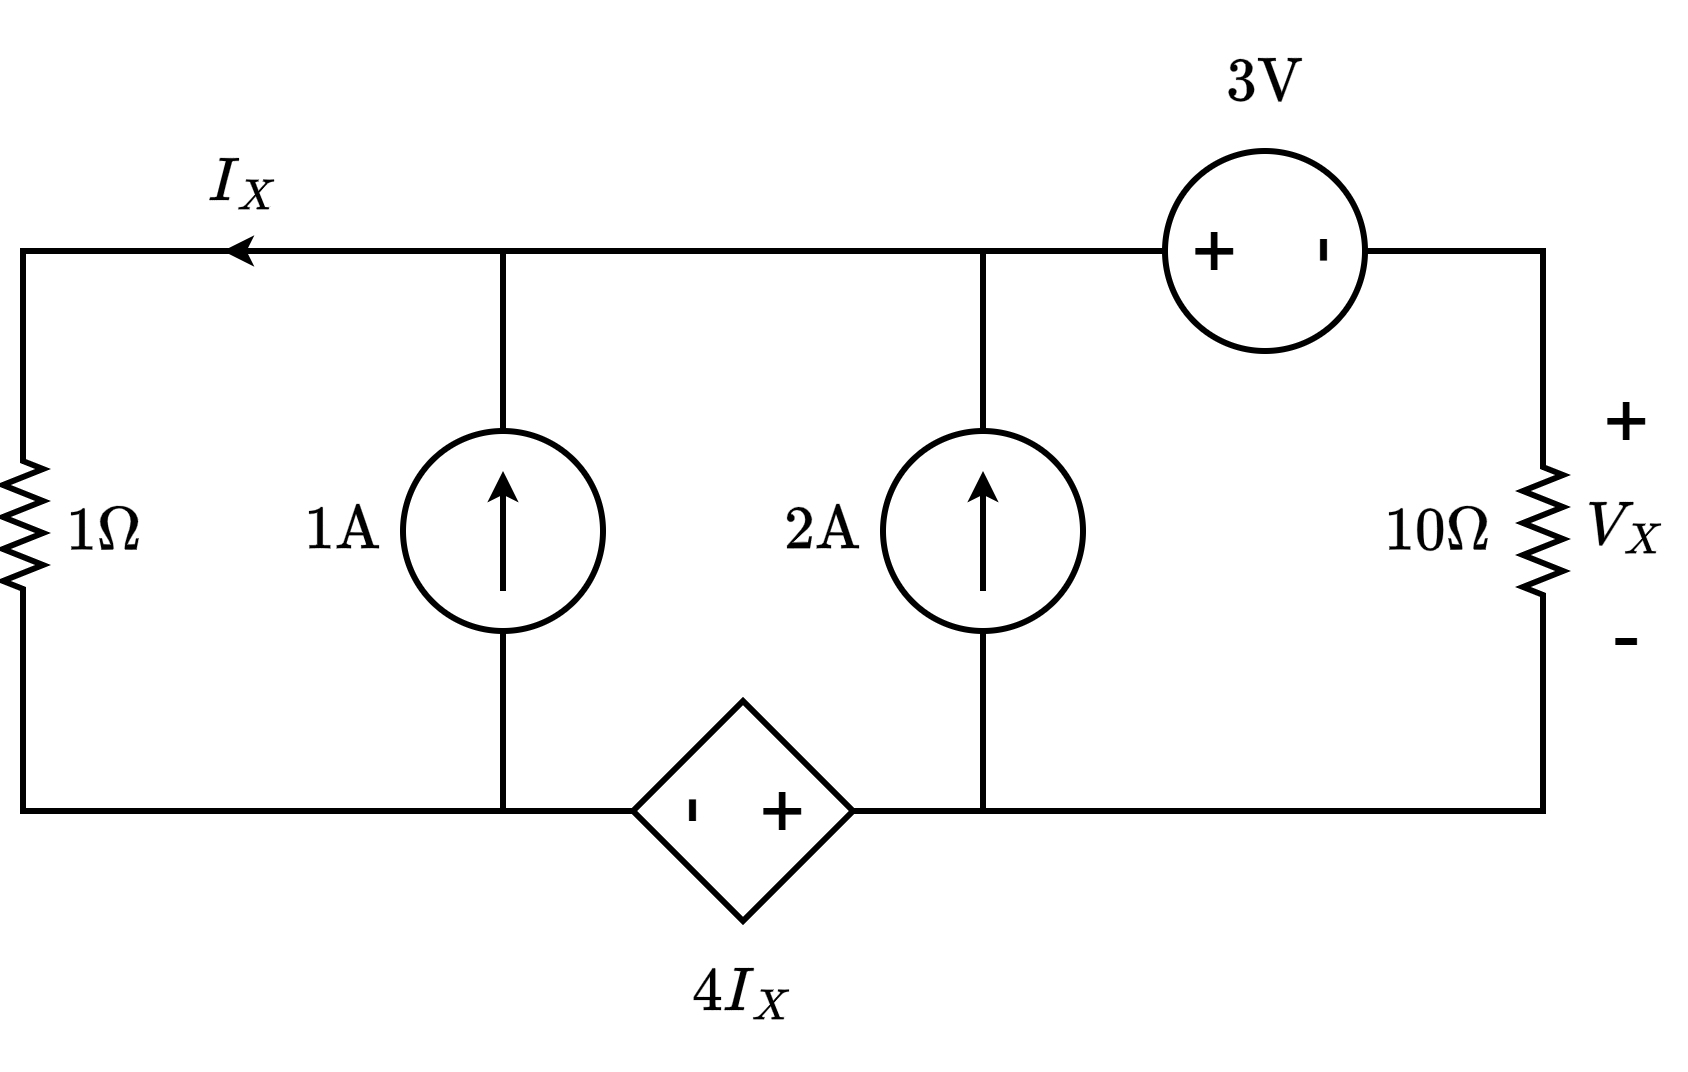
\includegraphics[width=5.2in]{schematic.png}
\end{center}

\begin{partquestion}{calculatevx}{Use superposition to determine $V_X$.}
\begin{answer}
Superposition tells us that we can consider the effect of each independent source individually. We can do this by disabling all but one of the independent sources (open current sources, short voltage sources) and solving for $V_X$. Keep in mind you shouldn't deactivate any dependent sources. Then we can add up all the results and we should get the final value of $V_X$.

\textbf{1 A source only:} open the 2 A source and short the 3 V source. The circuit becomes:
\begin{center}
    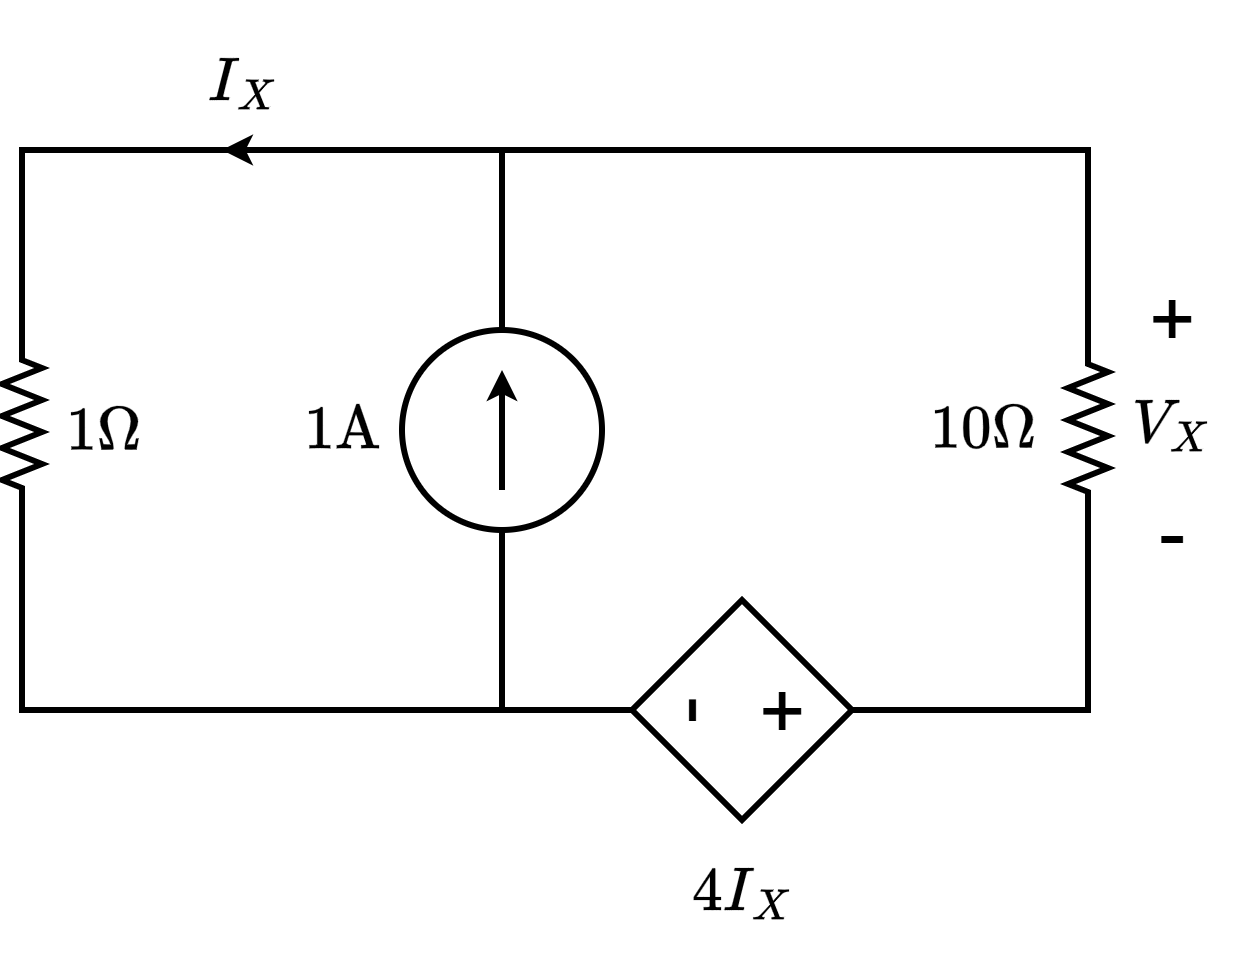
\includegraphics[width=3in]{super_1A.png}
\end{center}

KCL at the top node gives $1 = I_X + \frac{V_X}{10}$. KVL around the outer loop gives $V_X + 4 I_X - I_X = 0$, so $I_X = -\frac{V_X}{3}$. Substituting yields:
\[
1 = -\frac{V_X}{3} + \frac{V_X}{10} = -\frac{7}{30} V_X
\]
Thus $V_X = -\frac{30}{7}~\text{V}$.

\textbf{2 A source only:} open the 1 A source and short the 3 V source. The circuit becomes:
\begin{center}
    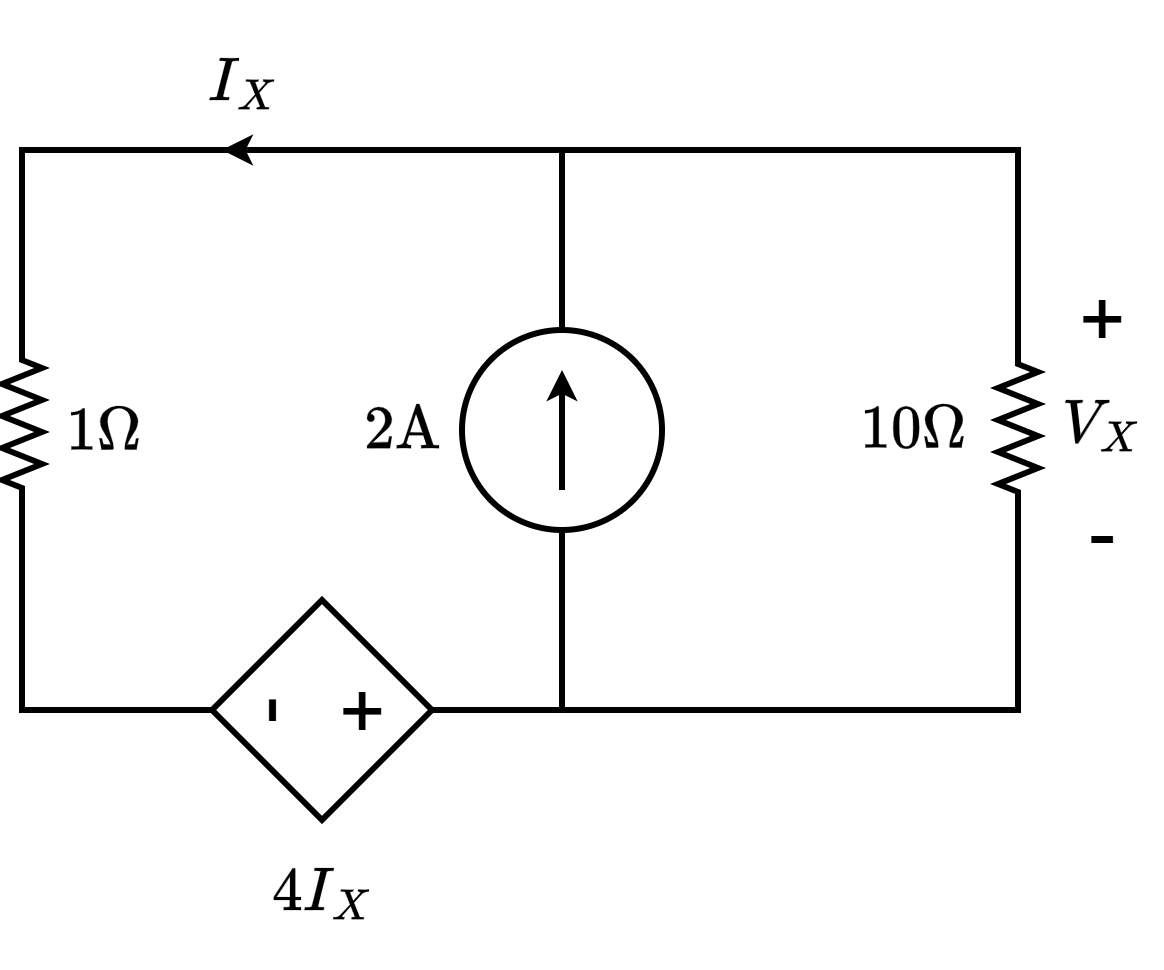
\includegraphics[width=3in]{super_2A.png}
\end{center}

KCL gives $2 = I_X + \frac{V_X}{10}$ and the same KVL relation $I_X = -\frac{V_X}{3}$. Therefore:
\[
2 = -\frac{V_X}{3} + \frac{V_X}{10} = -\frac{7}{30} V_X
\]
so $V_X = -\frac{60}{7}~\text{V}$.

\textbf{3 V source only:} open both current sources. The circuit becomes:
\begin{center}
    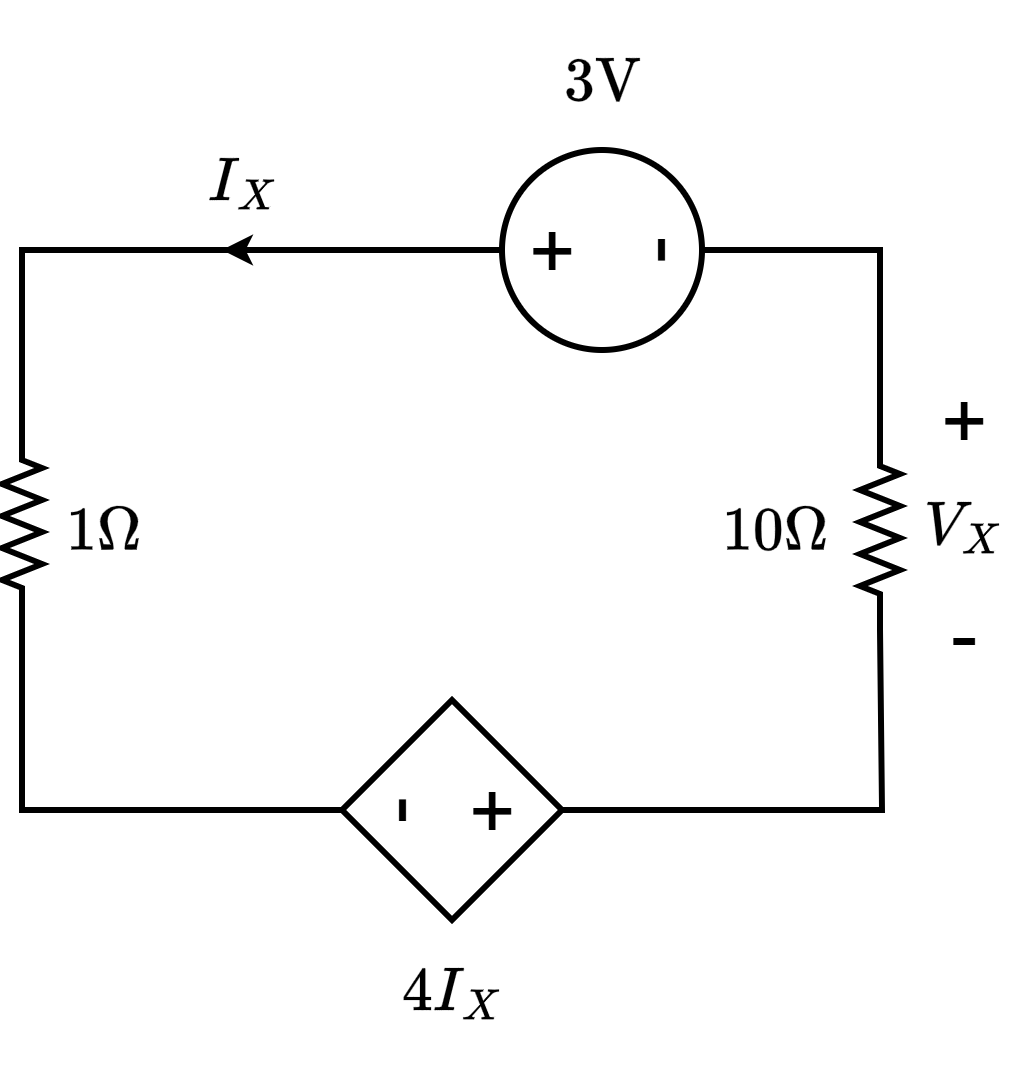
\includegraphics[width=3in]{super_3V.png}
\end{center}
The remaining loop gives $I_X(1) - 4 I_X - V_X - 3 = 0$ and, because the 10~$\Omega$ resistor carries $-I_X$, $V_X = -10 I_X$. Eliminating $I_X$ yields:
\[
\frac{3 V_X}{10} - V_X - 3 = 0
\]
so $V_X = -\frac{30}{7}~\text{V}$.

Superposition sums the contributions:
\[
V_X = -\frac{30}{7} - \frac{60}{7} - \frac{30}{7} = -\frac{120}{7} \approx -17~\text{V  } (\text{well maybe $-17.14$~V})
\]
\end{answer}
\end{partquestion}

\end{mainquestion}
